\subsection{Conversion}\label{ss:conversion}

Fig. \ref{fig:tosecmod} presents the conversion latency time from \secuint\ and \secint\ to \secmod\ for different bit sizes following the algorithms of Listings \ref{list:secuint2secmod} and \ref{list:secint2secmod}. The number of multiplications for \secuint\ and \secint\ stays constant at 0 and 2, while the multiplicative depth is 0 and 1, respectively, for all bit sizes. 
\iffalse As discussed in Section \ref{ss:bridging}, converting from \secint\ is slower than converting from \secuint\ because a \secint\ to \secmod\ conversion uses two ciphertext multiplications to account for the sign \fi . As expected, conversion from both \secuint\ and \secint\ becomes slower for larger bit sizes due to the larger number of additions required. The slowdown is the same for both types. It is less noticeable for \secint\ due the log-scale graph and the fact that the multiplications dominate the \secint\ latency time.

\begin{figure}[t]
	\centering
    \frame{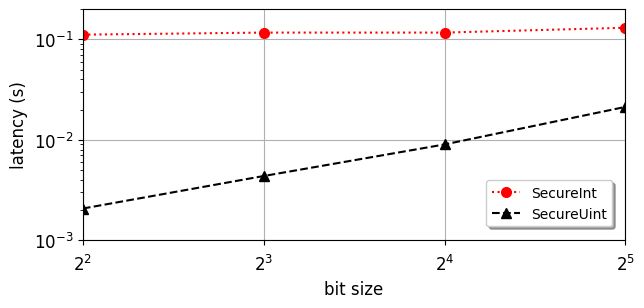
\includegraphics[width=\linewidth]{img/toSecureMod.png}}
	\caption{Conversion latency time from \secuint\ and \secint\ to \secmod\ for different bit sizes. Throughput is up to $n=2^{15}$ times faster since a ciphertext fits $n$ plaintexts.}
	\label{fig:tosecmod}
	\vspace{-0.6cm} 
\end{figure}

We also evaluate the conversion latency time from \secmod\ to \secuint/\secint\ using the algorithms presented in Listings \ref{list:secmod2secuint} and \ref{list:secmod2secint} with different plaintext moduli and bit sizes ($s = \{4, 8, 16, 32\}$). Fig.~\ref{fig:fromsecmod} summarizes the findings.
The results are what we expect from analysing the algorithms in Listings \ref{list:secmod2secuint} and \ref{list:secmod2secint}: When converting from \secmod\ to \secuint, the latency increases linearly to the bit size due to the operation on line 11 of Listing \ref{list:secmod2secuint}. Nevertheless, the dominant factor is the plaintext modulus $t$. A minor logarithmic effect comes from the exponentiation function (line 10) where the number of multiplications increases, while a major linear effect comes from the larger number of iterations in the \texttt{for} loop (line 7).
The conversion from \secmod\ to \secint\ (Listing \ref{list:secmod2secint}) takes roughly twice the time since it consists of two calls to the \secmod\ to \secuint\ conversion (lines 4 and 8) plus two multiplications (line 11).

\begin{figure}[t]
	\centering
    \frame{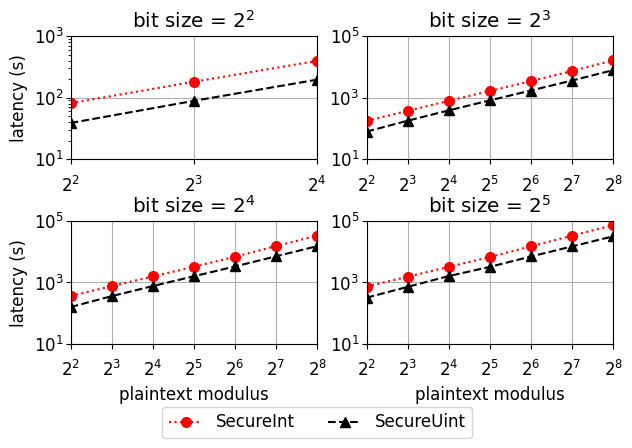
\includegraphics[width=\linewidth]{img/fromSecureMod.png}}
	\caption{Conversion latency time from \secmod\ to \secuint\ and \secint\ for different plaintext moduli and bit sizes.}
	\label{fig:fromsecmod}
	\vspace{-0.5cm}
\end{figure}



% \innersection{Insights}
% The results show that the conversion from bit-level to modular arithmetic is fast and can be used in practice. Meanwhile, converting from modular to bit-level arithmetic has borderline practical times only for very small plaintext moduli. With an small increase in the plaintext modulus, it quickly becomes prohibitive.
